%This is a experiment example of ZhengXiaoyang's experiment report template

\documentclass[UTF8]{ctexart}
\usepackage{pythonhighlight}
\usepackage{amsmath}
\usepackage{cases}
\usepackage{cite}
\usepackage{xeCJK}
\usepackage{graphicx}
\usepackage{siunitx}
\usepackage[margin=1in]{geometry}
\geometry{a4paper}
\usepackage{fancyhdr}
\pagestyle{fancy}
\fancyhf{}

\graphicspath{{picture/}}


\title{RLC电路暂态特性测量实验}
\graphicspath{{picture/}}


\title{RLC电路暂态特性测量实验报告}
\author{郑晓旸}
\date{\today}
\pagenumbering{arabic}

\begin{document}
%这里是文件的开头
\fancyhead[L]{郑晓旸}
\fancyhead[C]{RLC暂态}
\fancyfoot[C]{\thepage}

\maketitle
\tableofcontents
\newpage

\section{实验目的}

本实验的目的如下:
\begin{enumerate}
    \item 深入理解电路暂态过程的特点。
    
    通过观察和分析RC、RL和RLC电路在突变激励下的响应,了解电路暂态过程的特点,如一阶电路的指数衰减、二阶电路的阻尼振荡等,加深对电路暂态行为的理解。

    \item 掌握用示波器观察和测量暂态信号的方法。
    
    学习使用示波器捕捉和观察电路的暂态波形,包括合适的触发方式、耦合方式、时基和幅度设置等。同时,掌握从波形中测量暂态参数(如时间常数、振荡周期等)的方法,为以后的实验和工程实践奠定基础。
\end{enumerate}

\section{实验仪器}


本实验所需的仪器设备如下:

\begin{tabular}{rl}
    数字示波器 & 1台 \\
    信号发生器 & 1台 \\
    直流稳压电源 & 1台 \\
    数字万用表 & 1台 \\
    电阻箱 & 1个 \\
    电感器 & 1个 \\
    电容器 & 1个 \\
    面包板 & 1个 \\
    连接导线 & 若干
\end{tabular}

\begin{itemize}
    \item 数字示波器:用于观察和测量电路的暂态波形,示波器的带宽应满足测量要求。
    \item 信号发生器:提供方波或矩形波信号,触发电路暂态过程。信号发生器的上升/下降时间应尽量短,以获得理想的阶跃激励。
    \item 直流稳压电源:为电路提供稳定的直流电压。
    \item 数字万用表:测量电路中的直流电压、电流等参数,辅助计算电路元件的参数值。
    \item 电阻箱、电感器和电容器:构成被测试的RC、RL和RLC电路。元件参数应满足实验要求,且已知其标称值。
    \item 面包板和连接导线:搭建实验电路,连接各个元件和仪器设备。导线应有适当的长度和粗细,以减小杂散效应。
\end{itemize}
\newpage
\section{实验原理}

\subsection{RC和RL电路的暂态过程}

RC电路和RL电路是一阶动态电路,它们的暂态过程可以用一阶微分方程描述。当施加阶跃激励时,电路的响应为指数函数。

对于RC电路,放电时电容两端电压$u_C(t)$的变化规律为:
\begin{equation}
    u_C(t) = U_0 e^{-t/\tau}
\end{equation}
其中,$U_0$为阶跃激励的幅值,$\tau = RC$为时间常数。

对于RL电路,电感两端电压$u_L(t)$的变化规律为:
\begin{equation}
    u_L(t) = U_0 e^{-t/\tau}
\end{equation}
其中,$\tau = L/R$为时间常数。

通过示波器观察电容或电感两端的电压波形,可以验证以上规律,并测量时间常数$\tau$。

\subsection{RLC电路的暂态过程}

RLC电路是二阶动态电路,其暂态过程可以用二阶微分方程描述。当施加阶跃激励时,电路的响应取决于品质因数$Q$的大小。

当$Q > 1/2$时,电路为欠阻尼状态,电容两端电压$u_C(t)$的变化规律为:
\begin{equation}
    u_C(t) = U_0 (1 - \frac{1}{\sqrt{1-\zeta^2}} e^{-\zeta \omega_0 t} \sin(\omega_d t + \arccos(\zeta)))
\end{equation}
其中,$\zeta = 1/(2Q)$为阻尼比,$\omega_0 = 1/\sqrt{LC}$为固有角频率,$\omega_d = \omega_0 \sqrt{1-\zeta^2}$为阻尼角频率。

通过示波器观察电容两端的电压波形,可以验证以上规律,并测量阻尼振荡的周期$T$和衰减包络线的时间常数$\tau$,进而计算品质因数$Q$:
\begin{equation}
    Q = \frac{\pi}{\ln(\frac{u_C(t)}{u_C(t+T)})}
\end{equation}

当$Q$较小时,电路为过阻尼或临界阻尼状态,电容两端电压呈现非振荡的衰减过程。通过改变电路的阻尼(如改变电阻值),可以观察到不同阻尼状态下的暂态响应。
\newpage
\section{实验过程和数据分析}

\subsection{RC放电曲线的测量和时间常数计算}

首先,搭建RC串联电路,并使用方波信号触发电路的充放电过程。调节示波器的时基和电压灵敏度,观察并记录电容电压的波形。导出波形数据,使用Python程序进行数据处理和分析。

图\ref{fig:rc_discharge}显示了RC放电过程的电压波形。从图中可以看出,电容电压呈指数衰减,与理论分析一致。

\begin{figure}[htbp]
    \centering
    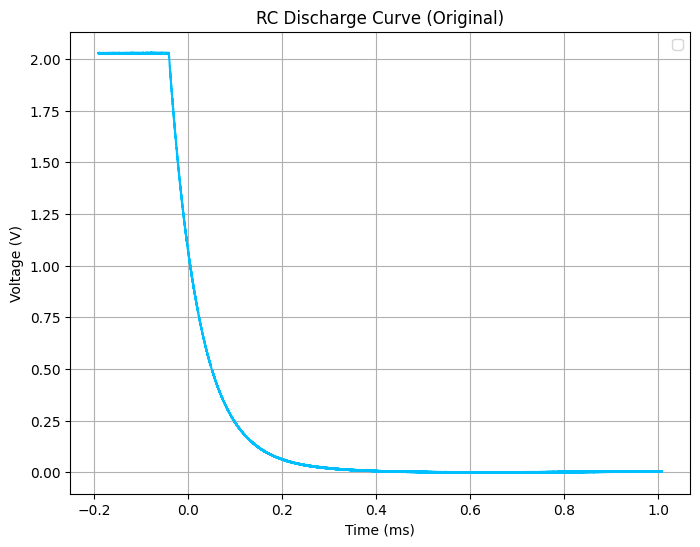
\includegraphics[width=0.5\textwidth]{rc_discharge.png}
    \caption{RC放电过程的电压波形}
    \label{fig:rc_discharge}
\end{figure}

通过对波形数据进行截取、滤波、指数拟合,如图\ref{fig:rc_discharge_preocessed},得到时间常数$\tau = \SI{0.068}{\ms}$。根据电路元件的测量值$R = \SI{13.2}{\ohm}$,信号发生器内阻$R_{gen} = \SI{50}{\ohm}$和$C = \SI{1}{\mu\farad}$,计算得到理论时间常数$\tau_{\text{theory}} =(R+R_{gen})C= \SI{0.063}{\micro\second}$。测量值与理论值的相对误差为$7.9\%$,误差较大。误差的主要来源可能是电容含有内阻,且电路内阻较大,以及电容的实际值与标称值有差异,以及示波器探头的影响。
\begin{figure}[htbp]
    \centering
    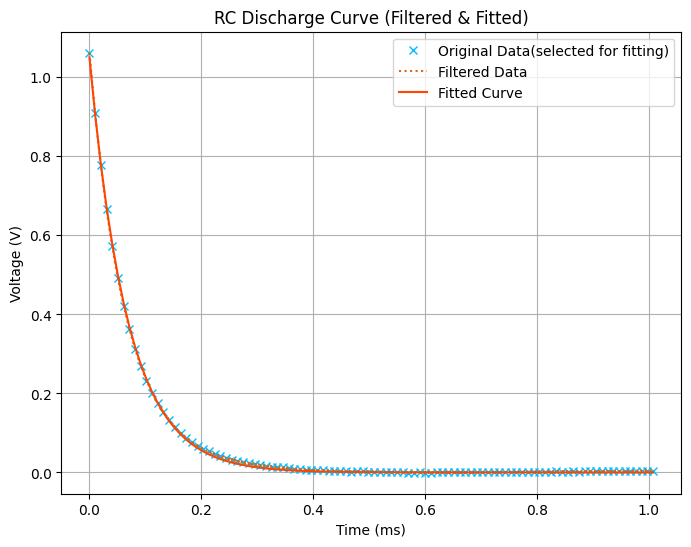
\includegraphics[width=0.5\textwidth]{rc_discharge_preocessed.png}
    \caption{RC放电过程的电压波形}
    \label{fig:rc_discharge_preocessed}
\end{figure}

\subsection{RLC欠阻尼振荡曲线的测量和参数计算}

接下来,搭建RLC串联电路,并使用方波信号触发电路的暂态过程。调节示波器的时基和电压灵敏度,观察并记录电容电压的波形。导出波形数据,使用Python程序进行数据处理和分析。

图\ref{fig:rlc_oscillation}显示了RLC电路欠阻尼振荡的电压波形。从图中可以看出,电容电压呈衰减振荡,振幅逐渐减小,与理论分析一致。

\begin{figure}[htbp]
    \centering
    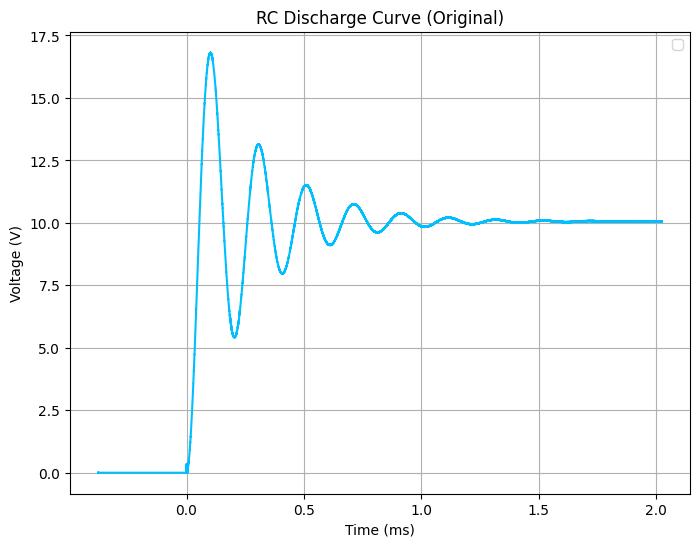
\includegraphics[width=0.5\textwidth]{rlc_oscillation.png}
    \caption{RLC欠阻尼振荡的电压波形}
    \label{fig:rlc_oscillation}
\end{figure}

通过测量相邻峰值之间的时间间隔,计算得到振荡周期$T = \SI{0.202}{\milli\second}$,对应的固有频率$f_0 = \SI{4.90}{\kilo\hertz}$。根据电路元件的标称值$L = \SI{10}{\milli\henry}$和$C = \SI{0.1}{\micro\farad}$,计算得到理论固有频率$f_{\text{theory}} = \SI{5.03}{\kilo\hertz}$,与测量值相对误差为$2.58\%$,误差较小,该误差可能由电路中串联产生的寄生电容以及并联示波器产生的电感产生。

通过对相邻峰值幅度的指数拟合,得到衰减系数$\alpha = 0.722$,由此计算品质因数$Q = \pi/\alpha = 4.352$。根据电路元件的单独测量值$L=\SI{10}{\milli\henry},C=\SI{0.1}{\micro\farad},R=\SI{1}{\ohm},R_{gen}=\SI{50}{ohm},R_{L}=\SI{14.3}{\ohm}$,计算得到理论品质因数$Q_{\text{theory}} = 4.86$,与测量值较为接近,误差为$10.85\%$。误差可能来自电阻值的不确定性和以及电感在高频震荡下的磁滞损耗所产生的等效电阻,这一点可以在进一步的测量中使用LC测试仪检测。
\\ 通过对波形数据进行截取、滤波、拟合和数据取点结果,如图\ref{fig:rlc_oscillation_processed}所示。
\begin{figure}[htbp]
    \centering
    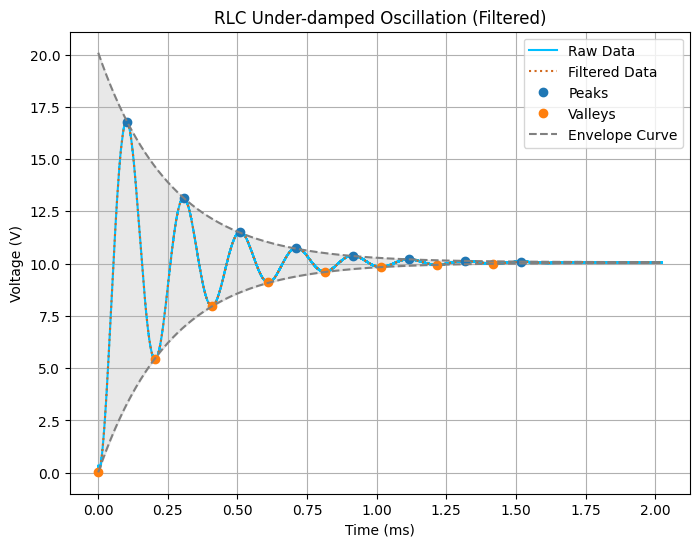
\includegraphics[width=0.5\textwidth]{rlc_oscillation_processed.png}
    \caption{RLC欠阻尼振荡的电压波形}
    \label{fig:rlc_oscillation_processed}
\end{figure}
\newpage
\subsection{RLC电路不同阻尼模式的观察和临界电阻测量}

最后,通过改变RLC电路中的电阻值,观察电路暂态过程的不同阻尼模式。当电阻较小时,电路表现为欠阻尼振荡;当电阻较大时,电路表现为过阻尼,电容电压单调衰减。通过调节介入电阻箱电阻值,找到临界阻尼状态,此时电容电压的衰减最快,无振荡,电阻箱阻值为$R_{box}=\SI{487}{\ohm}$。

实验测得临界电阻$R_c =R_{box} +R_{L}+R_{gen}= \SI{551.3}{\ohm}$。根据电感和电容的标称值,计算得到理论临界电阻$R_{c,\text{theory}} = 2\sqrt{L/C} = \SI{632.5}{\ohm}$,与测量值相差较大。这可能是由于电感和电容的实际值与标称值有差异,以及电路中的其他因素:电阻箱的内阻、电感的磁滞产生的等效电阻的影响。

图\ref{fig:rlc_damping}显示了RLC电路在三种不同阻尼状态下的电容电压波形。可以清楚地看到欠阻尼、临界阻尼和过阻尼的特点,与理论分析相符。

\begin{figure}[htbp]
    \centering
    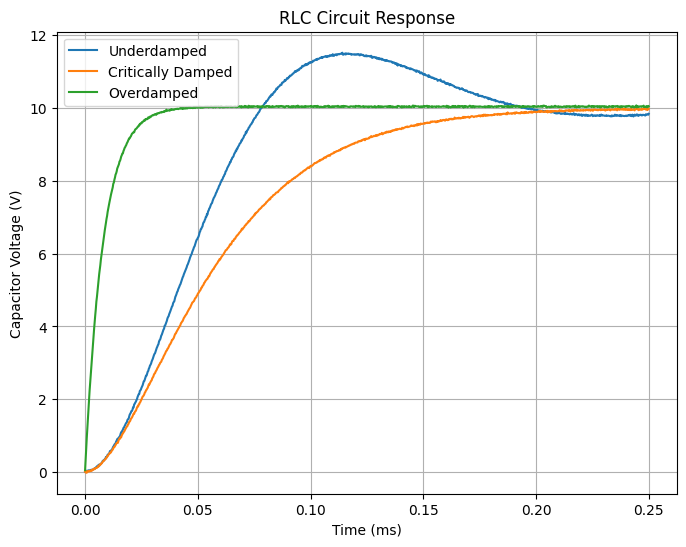
\includegraphics[width=0.5\textwidth]{rlc_damping.png}
    \caption{RLC电路在不同阻尼状态下的电容电压波形}
    \label{fig:rlc_damping}
\end{figure}
\section{分析与讨论}

\subsection{误差分析}
\section{实验误差和分析}

在本实验中,测量结果与理论值存在一定的误差。误差主要来源于随机误差和系统误差两个方面。

\subsection{随机误差}

在本实验中,可能的随机误差来源包括:

\begin{itemize}
    \item 示波器读数误差:由于示波器屏幕分辨率和人眼识别能力的限制,在读取电压和时间值时可能引入随机误差。
    \item 电路元件参数的波动:电阻、电容和电感的实际值可能在标称值附近波动,导致每次测量结果略有不同。
    \item 环境噪声干扰:外部电磁干扰和实验室环境的噪声可能对电路产生随机影响,导致测量结果的波动。
\end{itemize}

为了减小随机误差的影响,可以采取以下措施:
\begin{itemize}
    \item 多次测量取平均:对同一个量进行多次独立测量,然后计算平均值,可以减小随机误差的影响。
    \item 提高示波器的分辨率:使用分辨率更高的示波器,可以减小读数误差。
    \item 选用稳定的电路元件:使用高精度、低漂移的电阻、电容和电感,可以减小元件参数波动的影响。
    \item 屏蔽外部干扰:使用屏蔽电缆和屏蔽盒,可以减小外部电磁干扰的影响。
\end{itemize}

\subsection{系统误差}

在本实验中,可能的系统误差来源包括:

\begin{itemize}
    \item 示波器探头的影响:示波器探头的输入电容和电阻会对被测电路产生负载效应,导致测量结果与理论值存在系统偏差。
    \item 电路元件的标称值误差:电阻、电容和电感的实际值与标称值之间可能存在系统偏差,导致计算得到的理论值与真实值不一致。
    \item 实验电路的杂散参数:实验电路中的导线电阻、分布电容以及寄生损耗等杂散参数会影响电路的实际行为,导致测量结果与理想模型存在系统偏差。
\end{itemize}

为了减小系统误差的影响,可以采取以下措施:
\begin{itemize}
    \item 使用高阻抗探头:选用输入电阻较大的示波器探头,可以减小探头对电路的负载效应。
    \item 校准电路元件:使用精密的LCR表或其他校准设备,测量电路元件的实际值,并在理论计算中使用实测值而非标称值。
    \item 优化实验电路:合理布局实验电路,尽量减小导线长度和回路面积,以减小杂散参数的影响。必要时,可以在理论模型中引入修正项,以补偿杂散参数的影响。
\end{itemize}

通过采取以上措施,可以有效地减小随机误差和系统误差的影响,提高实验测量结果的准确性和可靠性。在分析实验数据时,应该考虑到这些误差来源,并对测量结果的不确定性进行合理估计。


\newpage

\section{附录}
\subsection{代码}
\subsubsection{RC放电过程的数据处理和分析}
\begin{python}
#C=1uF,R=10ohm,R_gen=50ohm
#U = U_C
import numpy as np
import pandas as pd
import matplotlib.pyplot as plt
from scipy.signal import savgol_filter
from scipy.optimize import curve_fit

# 读取CSV文件
original_data = pd.read_csv('RC_release1.csv')  
data = original_data[original_data['in s'] > 0]
# 提取时间和电压数据
time = 1000*data['in s'].values
voltage = data['C1 in V'].values
plt.figure(figsize=(8, 6))
plt.plot(1000*original_data['in s'].values,original_data['C1 in V'].values, '-',color = 'deepskyblue')
plt.xlabel('Time (ms)')
plt.ylabel('Voltage (V)')
plt.title('RC Discharge Curve (Original)')
plt.legend()
plt.grid(True)
plt.show()
# 使用Savitzky-Golay滤波器平滑数据
filtered_voltage = savgol_filter(voltage, window_length=51, polyorder=3)



# 定义指数衰减函数
def exp_decay(t, a, b):
    return a * np.exp(-b * t)

# 选取部分数据进行拟合
time_list=np.linspace(0, len(time)-1, num = 100,dtype=int)
fit_time = time[time_list]
fit_voltage = filtered_voltage[time_list]

# 拟合数据
popt, pcov = curve_fit(exp_decay, fit_time, fit_voltage)
a, b = popt
tau=1/b
# 绘制滤波后的数据图
plt.figure(figsize=(8, 6))
plt.plot(time[time_list], voltage[time_list], 'x',color = 'deepskyblue', label='Original Data(selected for fitting)')
plt.plot(time, filtered_voltage, ':',color = 'chocolate' , label='Filtered Data')
plt.plot(fit_time, exp_decay(fit_time, a, b), '-',color = 'orangered', label='Fitted Curve')
plt.xlabel('Time (ms)')
plt.ylabel('Voltage (V)')
plt.title('RC Discharge Curve (Filtered & Fitted)')
plt.legend()
plt.grid(True)
plt.show()

print(f"Fitted Parameters: a = {a:.3f}, b = {b:.3f}")
print(f"Time Constant (tau) = {(tau):.3f} ms,theory=0.06ms")



\end{python}
\subsubsection{RLC欠阻尼振荡过程的数据处理和分析}
\begin{python}
#C=0.1uf,L=10mH,R_gen=50ohm,R=15ohm
#U = U_C
import numpy as np
import pandas as pd
import matplotlib.pyplot as plt
from scipy.optimize import curve_fit
from scipy.signal import savgol_filter, find_peaks
# 读取CSV文件
original_data = pd.read_csv('RLC.csv')  
data = original_data[original_data['in s'] > 0]
# 提取时间和电压数据
time = 1000*data['in s'].values
voltage = data['C1 in V'].values
plt.figure(figsize=(8, 6))
plt.plot(1000*original_data['in s'].values,original_data['C1 in V'].values, '-',color = 'deepskyblue')
plt.xlabel('Time (ms)')
plt.ylabel('Voltage (V)')
plt.title('RLC Under-damped Oscillation (Original)')
plt.grid(True)
plt.show()

# 使用Savitzky-Golay滤波器平滑数据
filtered_voltage = savgol_filter(voltage, window_length=3000, polyorder=3)


# 找到滤波后数据的峰值和谷值
n=8
peaks, _ = find_peaks(filtered_voltage,height=voltage[-1],distance = 1000)
valleys, _ = find_peaks(-filtered_voltage,height=-voltage[-1],distance = 1000)
peaks = peaks[0:n]
valleys = valleys[0:n]

# 计算相邻峰值之间的时间差
peak_times = time[peaks]
valley_times = time[valleys]
periods = np.diff(peak_times)
avg_period = np.mean(periods)
print('T is ',avg_period)
# 计算固有频率
f0 = 1 / avg_period

# 计算峰谷值的幅度
peak_values = filtered_voltage[peaks]
valley_values = filtered_voltage[valleys]
peak_amplitudes = peak_values - voltage[-1]
valley_amplitudes =  voltage[-1] - valley_values
amplitudes = np.concatenate([peak_amplitudes, valley_amplitudes])
amp_time = np.concatenate([peak_times, time[valleys]]) 
# 拟合幅度差的指数衰减
def exp_decay(x, a, alpha,c):
    return a * np.exp(-alpha * x) + c

xdata = np.arange(len(amplitudes))
popt, pcov = curve_fit(exp_decay, amp_time, amplitudes)
a, alpha, C = popt



# 计算品质因数
# 计算相邻峰值之间的振幅衰减比
#print(exp_decay(peak_times[:-1],a,alpha,C))
#print(exp_decay(peak_times[1:],a,alpha,C))
amplitude_ratios = exp_decay(peak_times[:-1],a,alpha,C) / exp_decay(peak_times[1:],a,alpha,C)
an = np.log(np.mean(amplitude_ratios))
# 计算每个振幅衰减比对应的Q值
Q_values = np.sqrt(np.pi**2 / an**2 -1/4)



print(f"Quality Factor (Q) = {Q_values:.3f}")
print(f'Alpha = {an:.3f}')
print(f"Natural Frequency (f0) = {f0:.3f} kHz")


# 绘制滤波后的数据图
plt.figure(figsize=(8, 6))
plt.plot(time, voltage, '-', label='Raw Data',color = 'deepskyblue')
plt.plot(time, filtered_voltage, ':',color = 'chocolate' , label='Filtered Data')
plt.plot(time[peaks], filtered_voltage[peaks], "o",label='Peaks')
plt.plot(time[valleys], filtered_voltage[valleys], "o",label='Valleys')
plt.plot(time, exp_decay(time, a, alpha, C)+voltage[-1], '--',color = 'gray',linewidth = 0.3, label='Envelope Curve')
plt.plot(time, - exp_decay(time, a, alpha, C)+voltage[-1], '--',color = 'gray',linewidth = 0.3)
plt.fill_between(time, exp_decay(time, a, alpha, C)+voltage[-1],- exp_decay(time, a, alpha, C)+voltage[-1],color = 'lightgray',alpha=0.6)
plt.xlabel('Time (ms)')
plt.ylabel('Voltage (V)')
plt.title('RLC Under-damped Oscillation (Filtered)')
plt.legend()
plt.grid(True)
plt.show()




\end{python}
\subsection{原始数据}
见附件
\bibliographystyle{plain}
\bibliography{./template}  %bib文件名

\end{document}
